\documentclass[a4paper]{article}
\usepackage[utf8]{inputenc}  % si utf8
\usepackage{graphicx}
\usepackage{verbatim}

\pagestyle{plain}

\title{\textbf{Rapport de projet}\\- \Huge{Incidence} -}
\author{\emph{CHAMBONNET Kevin}\\\emph{GAUTHIER Silvère}\\\emph{MARTINEZ Thierry}\\\emph{MOKHRETAR Amin}}
\date{\today}

\newcommand{\alinea}{\hspace*{0.5cm}}

\begin{document}
  \maketitle
  \newpage
  \tableofcontents
  
  \newpage
  \part{Remerciements}

  \newpage
  \part{Cahier des charges}
  
    \section{Introduction}
      \subsection{Philosophie}
        \alinea Du point de vue d’un observateur, un monde peut être qualifié de complexe sans que les individus y évoluant ne le soient forcément. Dans ce TER, il est question d’aborder cette thématique sous forme de jeu. Autrement dit, le problème qui nous intéresse ici est de déterminer comment faire émerger un comportement global en mettant en oeuvre des contraintes extérieures dans l’environnement pour influencer les interactions locales d’agents. De plus il faudra, pour le joueur, analyser le comportement des ces derniers afin d’optimiser la réalisation des buts demandés. Plus précisément, il s’agit de mettre en scène des agents (disposant d’un comportement précis et défini en terme d’interaction), évoluant dans un environnement modifiable par un joueur humain (qu’il s’agisse d’ajouter des ressources exploitables, de modifier le relief, etc.) devant atteindre un certain objectif (stabilité du système écologique, récolte d’une certaine quantité de ressources, développement d’un chemin).

      \subsection{Questions fréquentes}
        \subsubsection{Qu'est-ce que ce jeu ?}
          \alinea C'est un jeu de type God-Like dans lequel on doit aider une civilisation à survivre le plus longtemps possible grâce à différents pouvoirs et actions divines.
			
        \subsubsection{Qu'est-ce que je contrôle ?}
          \alinea Vous ne contrôlez rien directement, tout se fait de façon indirecte grâce aux pouvoirs. Modifier l'environnement et aider les citoyens sont des actions qu'il faudra effectuer pour faire survivre la civilisation.
    
    \section{Mecanismes de jeu}
      \subsection{Jouabilité}
        \subsubsection{Conditions de victoire et de défaite}
          \alinea Il n'y aura pas de condition de victoire particulière dans le jeu de base, le but sera de survivre le plus longtemps possible.\\
          La partie se terminera quand le joueur n'aura plus de citoyen.
        \subsubsection{Sauver et Charger une partie}
          \alinea Le joueur pourra sauvegarder sa partie à tout moment, mais la sauvegarde se fera au moment de la dernière nuit.\\
          Le chargement d'une partie placera donc le joueur soit au début de la partie soit à la dernière nuit passée, avec la possibilité de modifier de nouveau les différentes options du jour (météo, métiers...).

%Multijoueur ? Mods ?
%Différent modes de jeu ?
%On peut créer ses propres cartes ? un éditeur accessible ?
%Ajout script, perso, autre ?

	  \subsection{Actions du joueur}
        \subsubsection{Pouvoirs de base}
          \begin{itemize} \small
            \item \textbf{Placer un Arbre :} Fait apparaître un Arbre sur une case choisie. Coût : 3 PI.
            \item \textbf{Placer un Arbre Fruitier :} Fait apparaître un Arbre Fruitier sur une case choisie. Coût : 6 PI.
            \item \textbf{Placer de la Pierre :} Fait apparaître de la Pierre sur une case choisie. Coût : 5 PI.
            \item \textbf{Placer de l'Eau :} Fait apparaître de l'Eau sur une case choisie. Coût : 2 PI.
            \item \textbf{Placer une Falaise :} Fait apparaître une Falaise sur une case choisie. Coût : 7 PI.
            \item \textbf{Placer un Buisson :} Fait apparaître un Buisson sur une case choisie. Coût : 4 PI.
            \item \textbf{Placer de la Terre :} Fait apparaître de la Terre sur une case choisie, la Terre placée s'adapte en fonction des autres Terres autour. Coût : 2 PI.
          \end{itemize} \normalsize

        \subsubsection{Pouvoirs divins}
          \begin{itemize} \small
            \item \textbf{Soigner :} Améliore l'état de santé d'un citoyen. Coût : 50 PI.
            \item \textbf{Naissance :} Crée un citoyen supplémentaire, hors naissances quotidiennes. Coût : 200 PI.
          \end{itemize} \normalsize

        \subsubsection{Choix de la nuit}
          \begin{itemize} \small
            \item \textbf{Météo :} Le joueur peut choisir la météo du jour suivant (ensoleillée ou pluvieuse).
            \item \textbf{Métier :} Le joueur peut orienter la distribution des métiers, sans définir exactement la proportion de chaque métier.
          \end{itemize} \normalsize
    
    \section{Structure du jeu}
    
      \subsection{Moteur multi-agent}
        
      \subsection{Moteur de carte}
    
        \subsubsection{La carte}

          \alinea La carte sera composée de 150x150 cases, mais ne sera affiché à l'écran qu'une vingtaine de cases en largeur sur une quinzaine en hauteur. Le déplacement sur la carte pourra se faire grâce aux touches fléchées mais aussi en plaçant la souris sur un des bords de l'écran.\\
          Le joueur ne pourra pas voir au delà des limites des 150x150 cases composant la carte.

        \subsubsection{Les Cases}

          \alinea La carte sera découpée en cases. Chaque case aura un type de base en début de partie, qui pourra ensuite être modifié selon le déroulement du jeu (cf. section \ref{DiagCase}, page \pageref{DiagCase}). Un élément neutre est un type de case ne donnant pas lieu à une ressource quelconque.\\
          \newline
          \label{TabCase}
          \begin{small}
            \begin{tabular}{| c | c | c |p{5cm}|}
              \hline
              &  &  &  \\
              \textbf{Type de case} & \textbf{Ressources} & \textbf{Franchissable} & \textbf{Description}\\
              &  &  &  \\
              \hline
              Terre & - & Oui & Type par défaut.\\
              \hline
              Terre Aride & - & Oui & Terre ne pouvant pas être cultivée.\\
              \hline
              Terre Innondée & - & Oui & Terre ne pouvant pas être cultivée.\\
              \hline
              Terre Fertile & - & Oui & Terre pouvant etre cultivée pour devenir un \textbf{Champs}.\\
              \hline
              Champs & Nourriture & Oui & Terre cultivée possédant plusieurs stades de maturité. Le maximum atteint, la récolte peut être effectuée et offrir de la nourriture.\\
              & (1 à 3 unités) &  &  \\
              \hline
              Arbre & Bois & Non & Peut être coupé pour récolter du bois.\\
              & (3 unités) &  &  \\
              \hline
              Arbre Fruitier & Bois, Nourriture & Non & Peut être coupé pour récolter du bois et de la nourriture.\\
              & (2 unités de chaque) &  &  \\
              \hline
              Eau & - & Non & Des poissons peuvent s'y trouver permettant de récolter de la nourriture.\\
              \hline
              Pierre & Pierre & Non & Peut être cassée pour récolter de la pierre.\\
              & (2 unités) &  &  \\
              \hline
              Falaise & - & Non & Elément neutre. Peut faire apparaître de la pierre à ses pieds.\\
              \hline
              Buisson & Nourriture & Non & La récolte de ses baies permet d'obtenir de la nourriture.\\
              & (2 unités) &  &  \\
              \hline
            \end{tabular}
          \end{small}
    
        \subsubsection{Diagramme de transitions des différentes cases}
          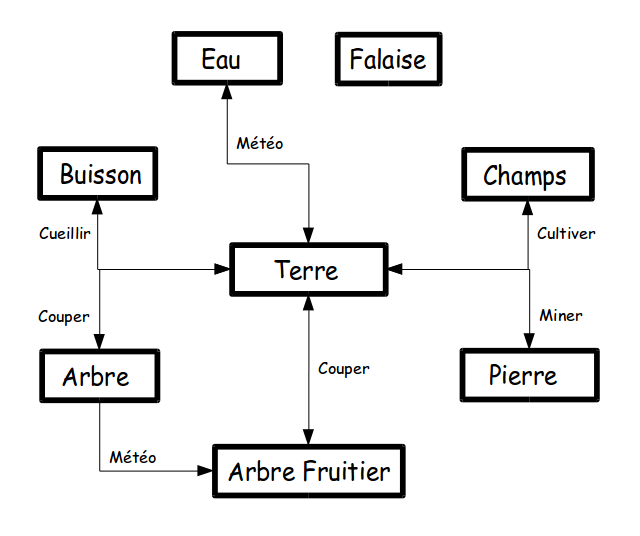
\includegraphics[scale=0.35]{img/DiagrammeTransitionCases.png} 
          \label{DiagCase}
        
        \subsubsection{Ressources utilisées par les citoyens}
          \alinea Ces ressources pourront être stockées dans une quantité illimitée, et les citoyens les utiliseront pour des constructions ou pour se nourrir.
          \begin{itemize} \small
            \item \textbf{Bois :} Utilisé pour la construction des bâtiments.
            \item \textbf{Pierre :} Utilisé pour la construction de certains bâtiments.
            \item \textbf{Nourriture :} Consommé par les citoyens chaque nuit pour se nourrir.
          \end{itemize} \normalsize
          \textbf{Comment ces ressources sont-elles récoltées ? }\\
          \alinea Elles sont récoltées par les citoyens, ainsi chaque métier correspond à la récolte d'une de ces ressources (cf. section \ref{Metier}, page \pageref{Metier}).

        \subsubsection{Ressources utilisées par le joueur}
          \alinea Cette ressource est la seule que le joueur pourra utiliser, elle sera stockée dans une quantité illimitée.
          \begin{itemize} \small
            \item \textbf{Point d'Incidence (PI) :} Utilisé à chaque action ou pouvoir divin.
          \end{itemize} \normalsize
          \textbf{Comment cette ressource est-elle récoltée ? }\\
          \alinea Elle sera obtenue grâce aux citoyens qui nous en feront gagner une petite quantité tout au long de leur journée. La nuit, chaque citoyen rapporte des points bonus.

        \subsubsection{La météorologie}
          \alinea La météo sera présente et sera contrôlée par le joueur. Elle aura une incidence sur l'environnement et les citoyens. Elle sera basique : ensoleillée ou pluvieuse, chacune des deux aura une incidence différente. 
          \begin{itemize} \small
            \item \textbf{Temps ensoleillé :} Améliore la pousse des champs mais un excès de soleil assèche les terres et récoltes, peut réduire les étendues d'eau et une sécheresse trop longue peut faire brûler certaines ressources.
            \item \textbf{Temps pluvieux :} Permet de faire pousser les champs. Un surplus de pluie innonde les terres et récoltes, augmente les probabilités de maladie et peut augmenter la taille des étendues d'eau.
          \end{itemize} \normalsize


        \subsubsection{Le cycle jour/nuit}
          \label{Cycle}
          \alinea Un cycle jour/nuit sera présent, avec des journées longues et des nuits courtes. Le Jour, les citoyens se vouent à leur métier, jusqu'au soir. La Nuit, tous les citoyens retournent au village, plus aucune action n'est possible. Lorsque la nuit tombe, toutes les actions du jour ont une incidence sur la nature et les entités, et seront visibles au début de la nouvelle journée.
          \begin{itemize} \small
            \item Le terrain est mis à jour, toutes les actions de la journée auront une incidence sur l'environnement.
            \item Tous les citoyens se nourrissent, la nourriture diminue en fonction du nombre de citoyen \textit{(-3 de nourriture par citoyen)}. S'ils manquent de la nourriture, certains citoyens peuvent tomber malade.
            \item Certains citoyens tombent malade en fonction des anciennes météos.
            \item S'il y a assez de nourriture, de nouveaux citoyens peuvent naître.
            \item Gain des points bonus d'incidence en fonction de la taille de la population et de sa santé.
            \item Mise à jour du métier de chaque citoyen, choisi en fonction des choix du joueur et des besoins.
          \end{itemize} \normalsize

        \subsubsection{Les incidences sur l'environnement :}
          \begin{itemize} \small
            \item Une étendue d'eau peut faire apparaître des poissons.
            \item Une étendue d'eau peut faire apparaître de la végétation dans les environs.
            \item Une zone de végétation très dense augmente les chances de faire apparaître des animaux herbivores.
            \item Une grande concentration d'animaux herbivores peut faire apparaître des animaux carnivores.
            \item Une forêt très dense augmente les chances de faire apparaître des arbres fruitiers.
            \item Les falaises peuvent faire apparaître des pierres par éboulement.
            \item La météo peut modifier la taille des étendues d'eau, assécher ou humidifier la terre.
          \end{itemize} \normalsize
        
      \subsection{Scripts}
      
    \section{Elements graphiques}

      \subsection{Les tuiles}
        \label{Tuile}
        \alinea Les tuiles seront des images de 32x32 ou 16x16 pixels au format PNG.\\
        \begin{itemize} \small
          \item \textbf{Le sol :} Il y aura 16 tuiles pour chaque type de sol, correspondant à toutes les possibilités de jonction avec le type voisin. En effet, chaque type de sol ne pourra être en contact qu'avec deux types différents suivant l'ordre hiérarchique suivant :\\
          Eau $\rightarrow$ Terre innondée $\rightarrow$ Terre fertile $\rightarrow$ Terre $\rightarrow$ Terre aride
          \item \textbf{Les ressources :} Il y aura 4 tuiles pour chaque ressource, correspondant au type de sol sur lequel elle se trouve.
          \item \textbf{Les bâtiments :} Chaque bâtiment sera constitué d'un ensemble de tuiles.
        \end{itemize} \normalsize
  
      \subsection{Les entités}
        \alinea Chaque entité aura plusieurs positions possibles. Pour chacun d'elle, un ou plusieurs éléments graphiques seront créés.\\
        \textbf{Les positions basiques :} Face, dos, profil droit, profil gauche.\\
        \textbf{Les positions spécifiques :} Coupant du bois, ramassant des baies, chassant, cultivant, construisant, se déplaçant sans ressource, se déplaçant avec des ressources.
	
      \subsection{Interface utilisateur}
		%Ici c'est tout ce qui est lié aux boutons et interfaces que le joueur utilisera 
		
    \section{Elements sonores}
    

  \newpage
  \part{Gestion du projet}
    \section{Gestion de l'équipe}
      \alinea Tous les membres se connaissant et étant supposés être capable de travailler en équipe, nous n'avons fait aucune élection de chef de projet.\\
      \alinea Nous avons opté pour travailler de manière collégiale, et ainsi garder une cohésion de groupe sans pour autant avoir de hiérarchie instaurée au sein du groupe, qui pourrait au contraire déservir la réalisation de nos objectifs.\\
      \alinea Chaque membre a donc autant de pouvoir que les autres, et peut donc participer activement au projet, autant lors de la conception que du développement. Toutes les décisions seront prises suivant la majorité lors de votes.\\\\
      \alinea Pour ce qui est des réunions de projets, nous avons convenu avec notre tuteur d'une réunion, allant d'environ trente minutes à une heure, toutes les une à deux semaines, afin de mettre au point l'avancement du projet. En parallèle, tous les membres de notre équipe se retrouvent une fois par semaine afin de discuter des points clés effectués ou à venir, donner lieu aux votes pour les prises de décisions, ou encore, lors de la phase de développement, travailler en collaboration afin d'optimiser notre travail.\\\\
      \alinea Au niveau du travail collaboratif, nous avons mis en place un dépôt sur github, contenant tant la documentation telle que ce rapport que les sources de notre jeu. Par ailleurs, nous mettrons sur ce dépôt uniquement les fichiers sources, les images et les sons, mais en aucun cas les fichiers temporaires ou les exécutables. Un fichier "makefile" sera disponible pour quiconque voudrait compiler le programme chez lui. Les seuls fichiers binaires disponibles seront les PDF de la documentation, pour un soucis de facilité d'accès.

    \section{Découpage en tâches}
      \alinea Afin de préparer le développement du jeu, il était nécessaire de séparer les fonctionnalités les unes des autres. Nous avons abouti à ce diagramme, qui résume notre choix de découpage :\\
      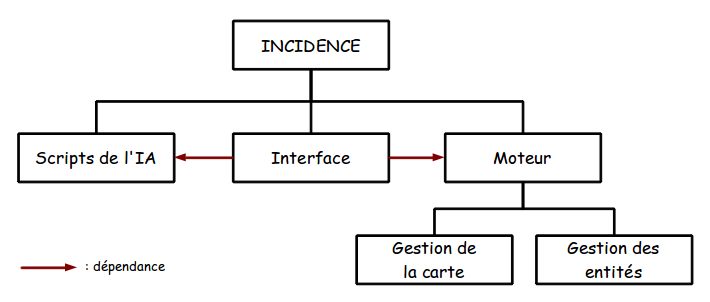
\includegraphics[scale=0.5]{img/DiagrammeDecoupageProjet.png}
      \label{DiagDecoupage}

    \section{Assignation}
      \alinea Le projet étant maintenant découpé en un certain nombre de modules, il ne restait plus qu'à assigner chaque tâche à un ou plusieurs membres de l'équipe. Nous nous sommes organisés comme ceci :
      \begin{itemize}
        \item \textbf{Scripts de l'IA :} MARTINEZ Thierry, MOKHRETAR Amin.
        \item \textbf{Moteur :}
        \begin{itemize}
          \item \textbf{Gestion de la carte :} GAUTHIER Silvère.
          \item \textbf{Gestion des entités :} CHAMBONNET Kevin.
        \end{itemize}
        \item \textbf{Interface :} Tous les membres.
      \end{itemize}
      \alinea Bien entendu, cette répartition n'est pas totalement fixée, elle concerne en réalité l'affectation de responsables de parties, qui seront en charge de celle-ci mais pourront évidemment faire appel aux autres membres pour trouver une solution à un problème par exemple.\\
      \alinea Le détail complet des tâches et assignations se situe dans la section Gestion du temps, page \pageref{GestionTps}.

    \section{Gestion du temps}
      \label{GestionTps}
      \alinea Afin de clarifier notre gestion du temps, un diagramme de Gantt est disponible en annexe et dans la documentation de notre projet, et sera mis à jour en fonction de l'avancée du projet.\\

    \section{Profil de risques}
      \begin{small}
        \begin{tabular}{| c | l |}
          \hline
          \textbf{Nature du risque} & \textbf{Degré du risque pour le projet}\\
          & 0 \hspace{0.5cm} 1 \hspace{0.5cm} 2 \hspace{0.5cm} 3 \hspace{0.5cm} 4 \hspace{0.5cm} 5\\
          \hline
          Taille du projet & \hspace{4.5cm} \circle*{5}\\
          \cline{1-1}
          Difficulté technique & \hspace{2.7cm} \circle*{5}\\
          \cline{1-1}
          Degré d'intégration & \hspace{2.25cm} \circle*{5}\\
          \cline{1-1}
          Configuration organisationnelle & \hspace{1.8cm} \circle*{5}\\
          \cline{1-1}
          Changement & \hspace{0.9cm} \circle*{5}\\
          \cline{1-1}
          Instabilité de l'équipe de projet & \hspace{0.9cm} \circle*{5}\\
          \hline
        \end{tabular}
      \end{small}

    \section{Choix technologiques}
      \subsection{Langages de programmation}
        \alinea Pour des besoins de performances, nous avons comparé différents langages. Pour réduire le temps de recherche et de comparaison, nous nous sommes appuyé sur des tests déjà effectués par d'autre.\\
        \alinea Des tests de performances concernant un large panel de langages, comparés dans quatre contextes différents, sont fournis en annexe.\\
        \alinea Nous pouvons observer que globalement, le langage le plus rapide est ici C++. L'utilisation de ce langage étant très fréquente dans les jeux vidéos, de part sa réputation d'un des langages les plus performants, et tous les membres de notre équipe sachant l'utiliser, nous avons fait le choix de programmer le moteur du jeu en C++.\\
        \alinea Afin d'optimiser encore la rapidité du moteur, nous avons cherché à associer son coeur écrit en C++ avec un langage de scripting qui permettra de mettre en place les différentes actions du jeu.\\ D'après les graphiques ci-dessus, nous avons opté pour le langage LUA, performant et facile d'utilisation (syntaxe proche du C++). En effet, même si Python est très prisé et offre beaucoup plus de possibilités que LUA, nous l'avons estimé bien trop lourd pour l'utilisation que nous allons en faire.\\
        \alinea Les deux langages C++ et LUA sont souvent associés dans les jeux vidéos, notre choix suit donc la tendance, ce qui nous offre une certaine assurance.

      \subsection{Bibliothèques}
        \alinea Pour la gestion graphique des tuiles composant la carte et des différentes entités, nous avons cherché une bibliothèque relativement simple d'utilisation mais surtout performante afin de garder la fluidité gagnée avec le choix des langages de programmation.\\
        \alinea Connaissant la bibliothèque OpenGL, qui est bas niveau et performante dans les affichages deux et trois dimensions, nous nous sommes tournés vers deux bibliothèques utilisant OpenGL : SDL et SFML.\\
        \alinea D'après plusieurs sites web et forums, les dernières versions (respectivement 2.0 et 2.1) de ces deux bibliothèques se valent en terme de performance.\\
        \alinea En confrontant nos préférences personnelles quant au choix de l'une ou l'autre, nous nous sommes finalement mis d'accord pour utiliser la bibliothèque graphique SFML 2.1, qui paraît plus simple d'utilisation que la SDL. De plus, elle permet une gestion aisée des fichiers audio, ce qui sera un plus pour la finalité de notre jeu.
      
    \section{Gestion des fichiers}
      \subsection{Format des Fichiers}
	    \alinea Le moteur de jeu étant écrit en C++, nous utiliserons des fichiers d'en-tête au format HPP et des fichiers de définition au format CPP. Pour les scripts d'IA des entités, le langage étant Lua, ceux-ci seront au format LUA.\\
        \alinea Toutes les images nécessaires au jeu seront au format PNG afin de pouvoir utiliser la transparence et garder la pleine qualité d'image (contrairement à JPEG qui perd de l'information à la compression).\\
        \alinea Les sons quant à eux seront au format WAV afin d'éviter toute gestion de la compression de fichier pour de petits fichiers qui n'en ont aucunement besoin.

        \subsubsection{Animation}
          \begin{verbatim}
            Chemin/vers/image.png size_x_sprite size_y_sprite play?(1/0) loop?(1/0)
            +Frame position_x position_y temps_affichage
            +Frame position_x position_y temps_affichage
            +Frame position_x position_y temps_affichage
          \end{verbatim}
      
        \subsubsection{Tileset}
	      \alinea Le tileset sera une unique image au format PNG représentant l'ensemble des tuiles possibles. Chaque type de sol constituera une ligne du tileset, avec toutes les variantes dépendant des rebords entre tuiles (ce fichier sera présenté plus en détails dans la section \ref{TilesetDev}, page \pageref{TilesetDev}).

        \subsubsection{Carte}
	      \alinea Les différentes cartes sauvegardées seront enregistrées dans des fichiers IMS (Incidence Map Save), dans lesquels seront stockés le tileset utilisé et la conformation de la carte (dimensions, sols et éléments).
      
        \subsubsection{Sauvegarde}
		  \alinea Un fichier sera créé pour la savegarde du jeu et un autre pour la sauvegarde de la carte, cela permettant dans le futur de créer des cartes réutilisables, comme par exemple dans un éditeur de carte.\\
		  \\
		  \alinea %TODO
		  \\
		  \alinea Le fichier de carte contiendra uniquement le lien vers le tileset ainsi que les types de sols et éléments présents sur la carte. Le fichier sera donc de la taille : 2 * nombre\_de\_cases * sizeof(int) + sizeof(chemin\_du\_tileset).\\
      
      \subsection{Commentaires}
        \alinea Si une méthode ou fonction, voir même un bloc, dépasse une certaine taille (environ 10 lignes) ou devient trop compliquée, un commentaire sera ajouté avant celle-ci expliquant brièvement son processus :
        \begin{verbatim}
          /** Description :
          *** Entrée : ...
          *** Sortie : ...
          **/
        \end{verbatim}
        \begin{small}
          \begin{tabular}{| c | c |}
            \hline
            \textbf{Marqueur spécifique} & \textbf{Signification}\\
            \hline
            TODO & A mettre à la place du code d'une fonctionnalité à implémenter\\
            \hline
            RECODE & A mettre au dessus du bloc d'une fonctionnalité à refaire\\
            \hline
            FIXME & A mettre au dessus du bloc d'une fonctionnalité contenant un bug\\
            \hline
          \end{tabular}
        \end{small}

      \subsection{Convention de Nommage}
        \begin{small}
          \begin{tabular}{| c | c |}
            \hline
            \textbf{Type de variable} & \textbf{Format du nom}\\
            \hline
            Classe & Majuscule suivit de minuscules\\
            \hline
            Méthode & Minuscules (pour les mots composés,\\
            et & chaque mots suivant est\\
            Fonction & une majuscule suivit de minuscules)\\
            \hline
            Attribut de classe & m\_\\
            \hline
            Variable globale & g\_\\
            \hline
          \end{tabular}
        \end{small}

      \subsection{Gestion du code source}
        \alinea Afin de faciliter le travail collaboratif, nous utilisons un dépôt utilisant le gestionnaire de version GIT, hébergé sur le site https://github.com/. Sur ce dépôt seront présents tous les fichiers sources nécessaires au développement du jeu ainsi que les documentations au format Latex et PDF (même si aucun fichier binaire ne devrait être présent, il est plus pratique de récupérer directement un tel fichier que de le compiler soit-même). De plus, y seront stockées toutes les données utilisées par le jeu telles que les images et les sons. Seuls les fichiers temporaires, exécutables et fichiers de sauvegarde ne seront pas stockés.
		

  \newpage
  \part{Développement}
  
    \section{Moteur de jeu}
    
      \subsection{Gestion des états}
      
      \subsection{Gestion de l'interface utilisateur}
      
      \subsection{Gestion des ressources et animations}
% 	    \alinea Tous les effets graphiques du projet sont à base de sprites. Nous avons initialement choisi des tuiles de 32x32 pixels, mais il serait possible de changer cette taille dans le futur.\\
%     	\\
%     	\alinea Chaque sol du tileset est affiché avec des bordures selon les types de sols environnant.\\
%       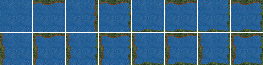
\includegraphics[scale=0.2]{img/groundSample.png}
%       \alinea Chaque élément est affiché différemment selon le type de sol sur lequel il se trouve.\\
%       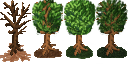
\includegraphics[scale=0.2]{img/elementSample.png}
%       \alinea Chaque entité est animée selon sa classe, son sens de déplacement ou son action.\\
%       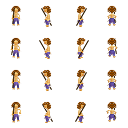
\includegraphics[scale=0.2]{img/animationSample.png}
      
	\section{Moteur de carte}
      \subsection{Les Tuiles}
        \alinea Les différents types de tuile seront tous recensés dans le tileset, qui se chargera de fournir les textures et attributs associés à ceux-ci. La carte n'utilisera que des pointeurs vers ces instances constantes de tuile, ce  qui évitera le stockage inutile d'instances identiques.
        
        \subsubsection{Les Sols}
          \alinea Chaque sol aura différents attributs définis dans le fichier de configuration du tileset (cf section \ref{TilesetDev}, page \pageref{TilesetDev}). Comme définis dans le cachier des charges, certains sols seront incompatibles avec d'autres.\\
          \\
	  	  \begin{small}
			\begin{tabular}{| c | l |}
			  \hline
			  \textbf{Attribut} & \textbf{Description}\\
			  \hline
			  Type & Entier définissant un identificateur du type de sol.\\
			  \hline
			  Coût & Entier définissant le coût en PI de la pose du sol.\\
			  \hline
			  Nom & Chaîne de caractères utilisées lors des affichages dans l'interface.\\
			  \hline
			  Comportement & Enumération de trois comportements :\\
			  & DEFAULT : comportement par défaut (tous les type de Terre).\\
			  & FLUID : les sols forment des zones (étendues d'eau).\\
			  & CLIFF : les sols sont fixes et forment des zones (falaises).\\
			  \hline
			  Franchissable & Booléen indiquant si le sol est franchissable ou non par les unités.\\
			  \hline
			  Rebords & Tableaux d'entiers indiquant tous les types de sol compatibles\\
			  & avec les bordures de l'image (cf  section \ref{TilesetDev}, page \pageref{TilesetDev}).\\
			  \hline
			\end{tabular}
		  \end{small}
          
        \subsubsection{Les Eléments}
          \alinea Chaque sol aura différents attributs définis dans le fichier de configuration du tileset (cf section \ref{TilesetDev}, page \pageref{TilesetDev}).\\
          \\
	  	  \begin{small}
			\begin{tabular}{| c | l |}
			  \hline
			  \textbf{Attribut} & \textbf{Description}\\
			  \hline
			  Type & Entier définissant un identificateur du type d'élément.\\
			  \hline
			  Type de sol & Entier définissant un identificateur du type de sol sur lequel se place l'élément.\\
			  \hline
			  Coût & Entier définissant le coût en PI de la pose de l'élément.\\
			  \hline
			  Nom & Chaîne de caractères utilisées lors des affichages dans l'interface.\\
			  \hline
			  Comportement & Enumération de deux comportements :\\
			  & DEFAULT : comportement par défaut.\\
			  & FOREST : les éléments forment des zones (arbres).\\
			  \hline
			  Franchissable & Booléen indiquant si le sol est franchissable ou non par les unités.\\
			  \hline
			  Temps de récolte & Valeur de temps durant laquelle le citoyen doit agir afin de récolter les ressources.\\
			  \hline
			  Ressources & Ressources (et leur quantité) associées à l'élément.\\
			  \hline
			\end{tabular}
		  \end{small}
          
          
      \subsection{Le Tileset}
		\label{TilesetDev}
		\alinea Un unique fichier image au format PNG contiendra l'ensemble des tuiles utilisées dans le jeu pour les sols ou éléments. Cette image sera utilisée comme texture et certaines parties seront extraites par le programme au gré des besoins.
		\alinea Dans le but de permettre à l'utilisateur d'aisément créer des mods de jeu ou changer de tileset, nous avons créé un fichier au format INI détaillant toutes les particularités du tileset.\\
		\alinea Voici le tileset que nous utiliserons :\\
        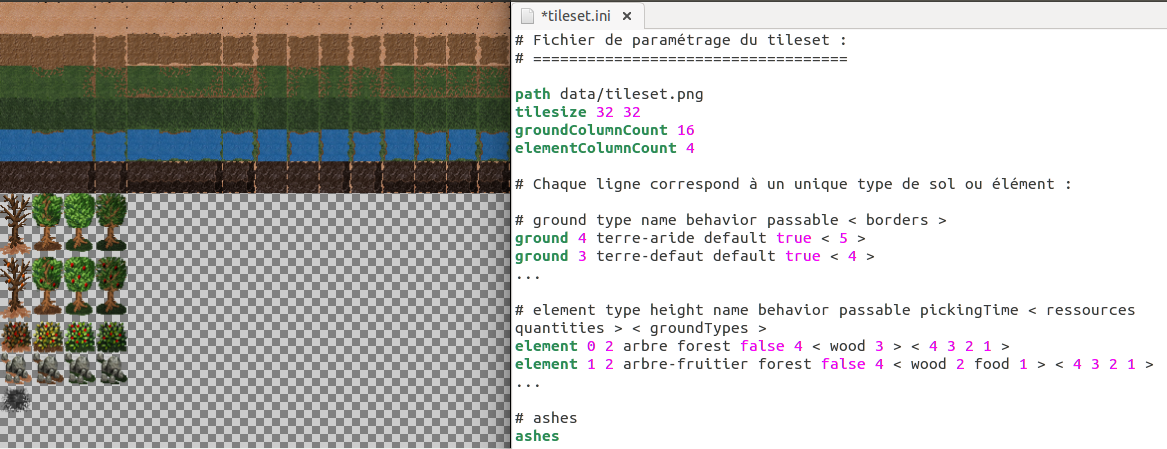
\includegraphics[scale=0.35]{img/TilesetPngIni.png}
        \label{TilesetPngIni}
        \\
        \textbf{Fichier de configuration :}\\
        \alinea Chaque ligne commençant par "\#" ne sera pas lue, ce sont les commentaires. Les mots en vert sont les mots clés utilisés pour la lecture qui se fait ligne par ligne :\\
        - path : indique le chemin du fichier de texture du tileset\\
        - tilesize : est suivi des dimensions (en pixel, largeur puis hauteur) d'une tuile\\
        - groundColumnCount : nombre de colonnes pour chaque sol dans le fichier de texture (toutes les associations de rebords)\\
        - elementColumnCount : nombre de colonnes pour chaque élément dans le fichier de texture (tous les types de sols)\\
        - ground : définit un sol et tous ses attributs\\
        - element : définit un élément et tous ses attributs (height est la hauteur en nombre de cases dans la texture)\\
        - ashes : fourni une texture pour les cendres (lorsque des éléments brûlent) (cf GDD)\\
        \\
        Remarque : chaque ligne commençant par ground, element ou ashes incrémente un compteur afin de connaître la position de la zone de texture correspondante. L'ordre est donc important (définition des lignes de haut en bas).

      \subsection{Météo}
      
      \subsection{Incidences}
        \subsubsection{Dilatation}
          \alinea Les incidences basées sur la dilatation des zones prennent en compte les types de sols ou éléments afin d'élargir les étendues voulues en propageant les sols si besoin afin de garder les contraintes définies dans le GDD.\\
          \alinea Quelques présentations des résultats de ces dilatations sont présentes en annexe.\\
        
        \subsubsection{Erosion}
          \alinea Les incidences basées sur l'érosion des zones prennent en compte les types de sols ou éléments alentours afin de choisir les types en propageant les sols si besoin afin de garder les contraintes définies dans le GDD.\\
          \alinea Quelques présentations des résultats de ces érosions sont présentes en annexe.\\
        
        \subsubsection{Aléatoire}
          \alinea Les dernières incidences concernant le territoire sont basées sur un choix aléatoire de cases. Il s'agit ici d'appartition ou disparition de certaines ressources.\\
          \alinea Quelques présentations des résultats de ces incidences particulières sont présentes en annexe.\\

	\section{Moteur multi-agent}
	
		\subsection{Gestion des entités}
		
			\subsubsection{Santé}
			
			\subsubsection{Incidences}
			
		\subsection{Gestion des scripts}
		
		\subsection{Liste des scripts}
		
	\section{Architecture}
	
		\subsection{Machine à états}
			pour chaque etat :
			interface + graphiques + sons + action possibles
	

  \newpage
  \part{Post-Mortem}
  
	\section{Réalisations non abouties}
	
	\section{Améliorations réalisables}
	

  \newpage
  \part{Annexes}
    \alinea Dans cette partie seront placés les éléments trop volumineux pour être inclus directement dans le texte, tels que les images ou graphiques.\\
    
    \section{Diagramme de Gantt}
      \alinea Le diagramme est fourni page \pageref{DiagGantt1} - \pageref{DiagGantt2}.
      \begin{figure}
        \begin{center}
          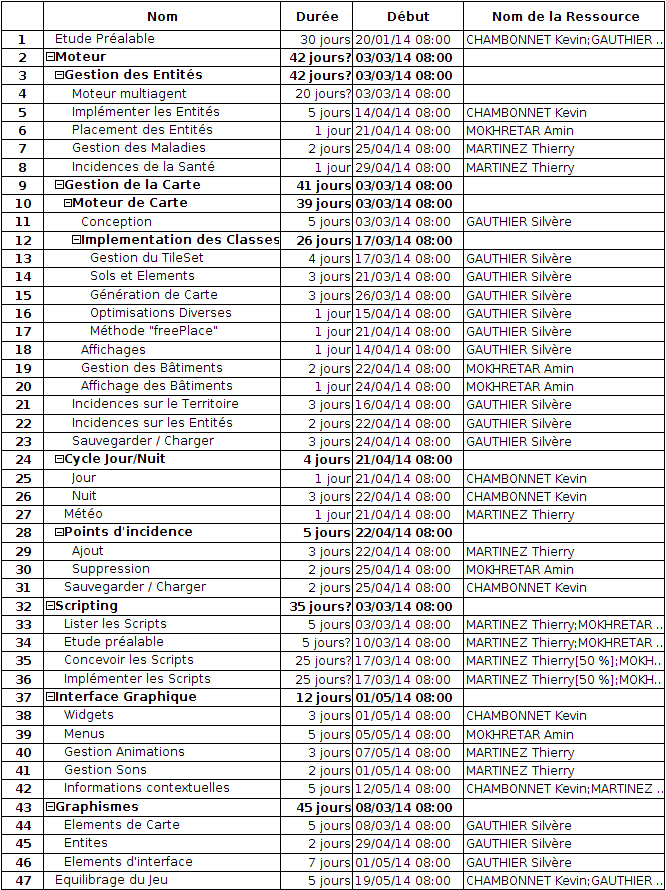
\includegraphics[scale=0.5]{img/gantt_1.png}
        \end{center}
        \label{DiagGantt1}
        \caption{Diagramme de Gantt (page 1)}
      \end{figure}
      \begin{figure}
        \begin{center}
          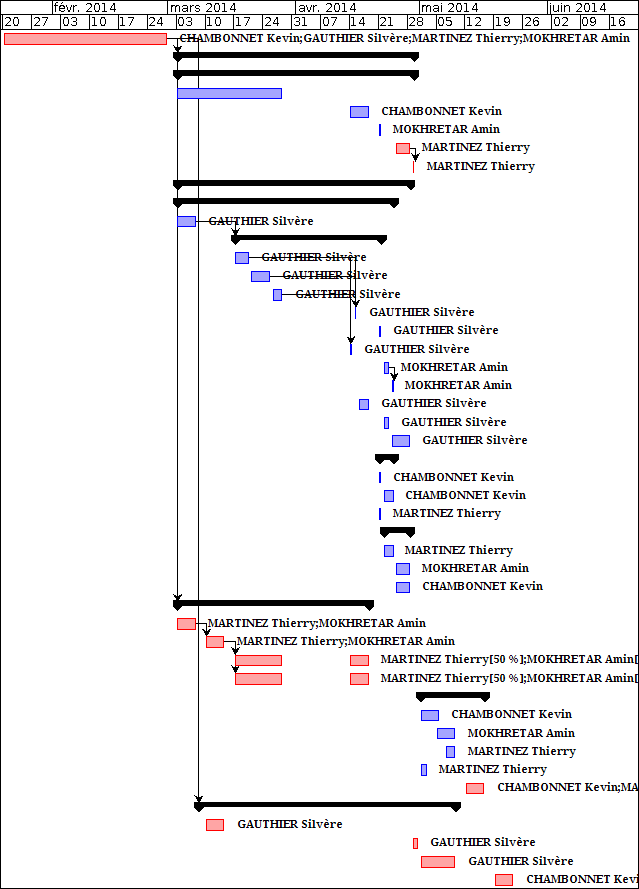
\includegraphics[scale=0.5]{img/gantt_2.png}
        \end{center}
        \label{DiagGantt2}
        \caption{Diagramme de Gantt (page 2)}
      \end{figure}
      
    \section{Comparatif de performances}
      \alinea Le graphique est situé page \pageref{DiagAnalyse}.
      \begin{figure}
        \begin{center}
          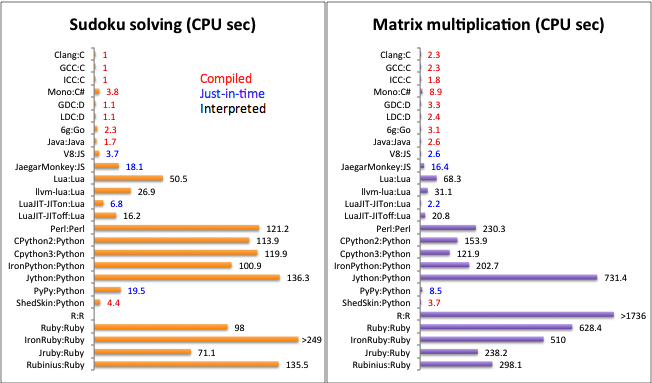
\includegraphics[scale=0.5]{img/AnalyseLangage1.png}
          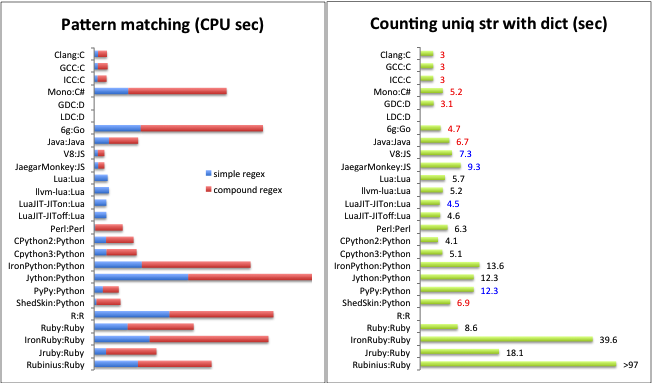
\includegraphics[scale=0.5]{img/AnalyseLangage2.png} 
        \end{center}
        \label{DiagAnalyse}
        \caption{Comparaisons de performances de divers langages dans des cas donnés}
      \end{figure}
      
    \section{Incidences sur la carte}
      \alinea Les présentations sont présentes de la page \pageref{IncidenceDeb} à la page \pageref{IncidenceFin}.
      \begin{figure}
        \begin{center}
          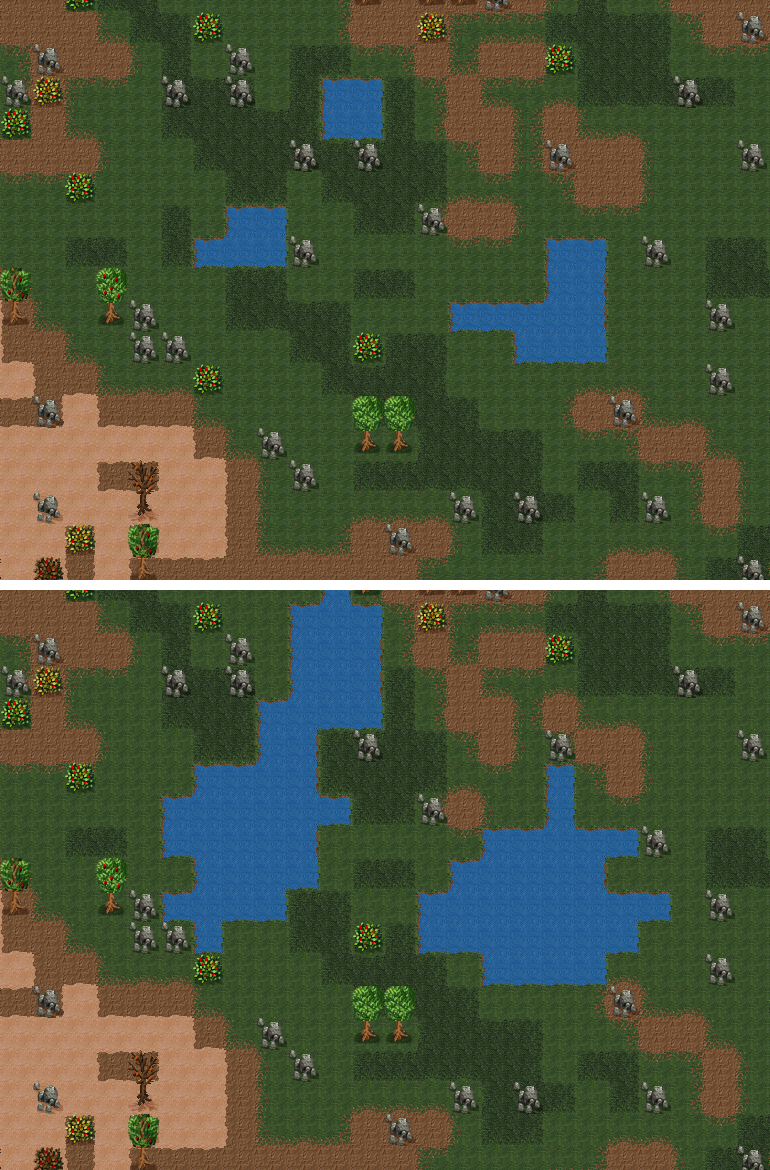
\includegraphics[scale=0.45]{img/DilateFluid.png}
        \end{center}
        \label{IncidenceDeb}
        \caption{Dilatation des étendues de fluides}
      \end{figure}
      \begin{figure}
        \begin{center}
          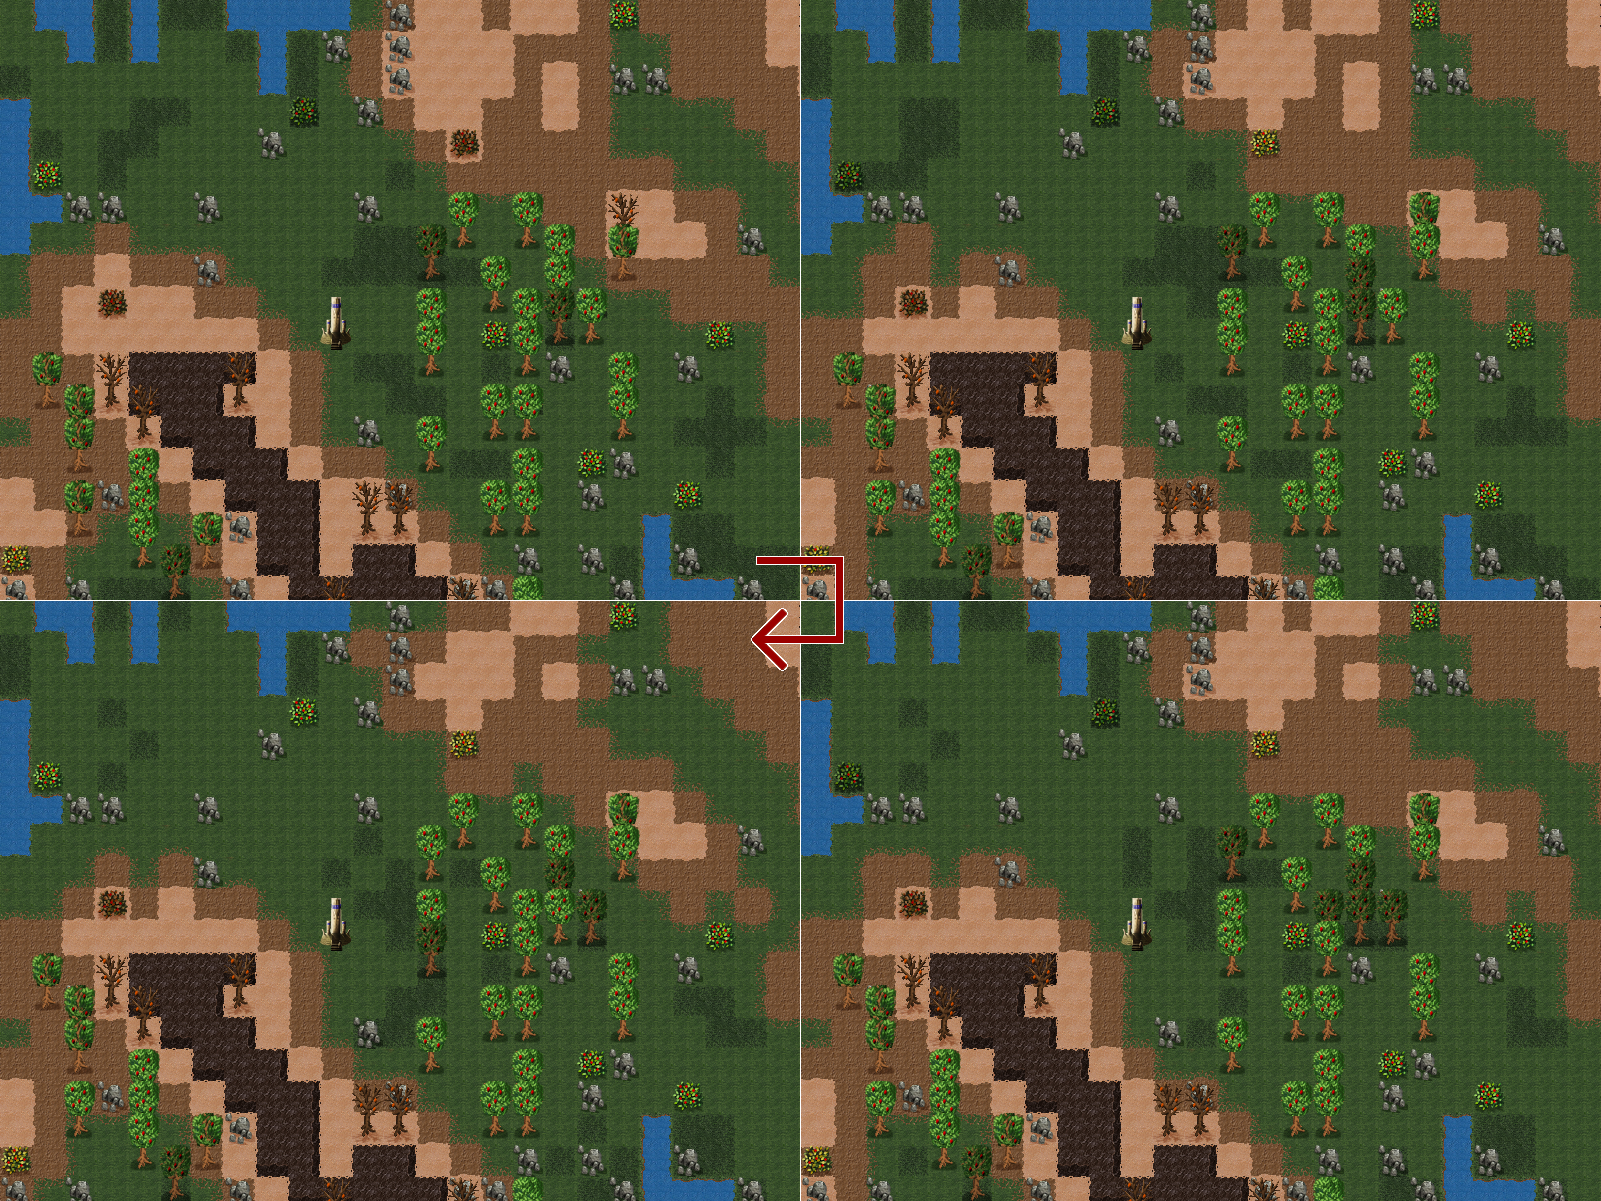
\includegraphics[scale=0.45]{img/DilateNearFluid.png}
        \end{center}
        \caption{Dilatation des zones humides}
      \end{figure}
      \begin{figure}
        \begin{center}
          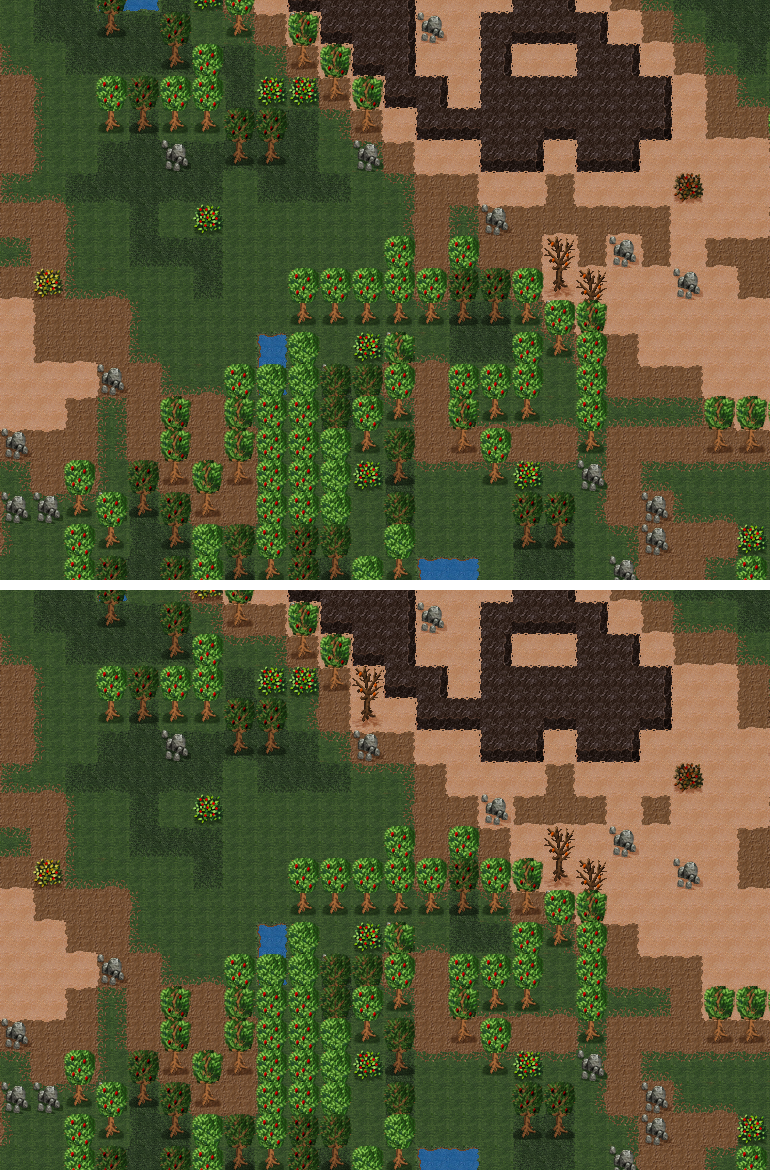
\includegraphics[scale=0.45]{img/DilateNearCliff.png}
        \end{center}
        \caption{Dilatation des zones sèches}
      \end{figure}
      \begin{figure}
        \begin{center}
          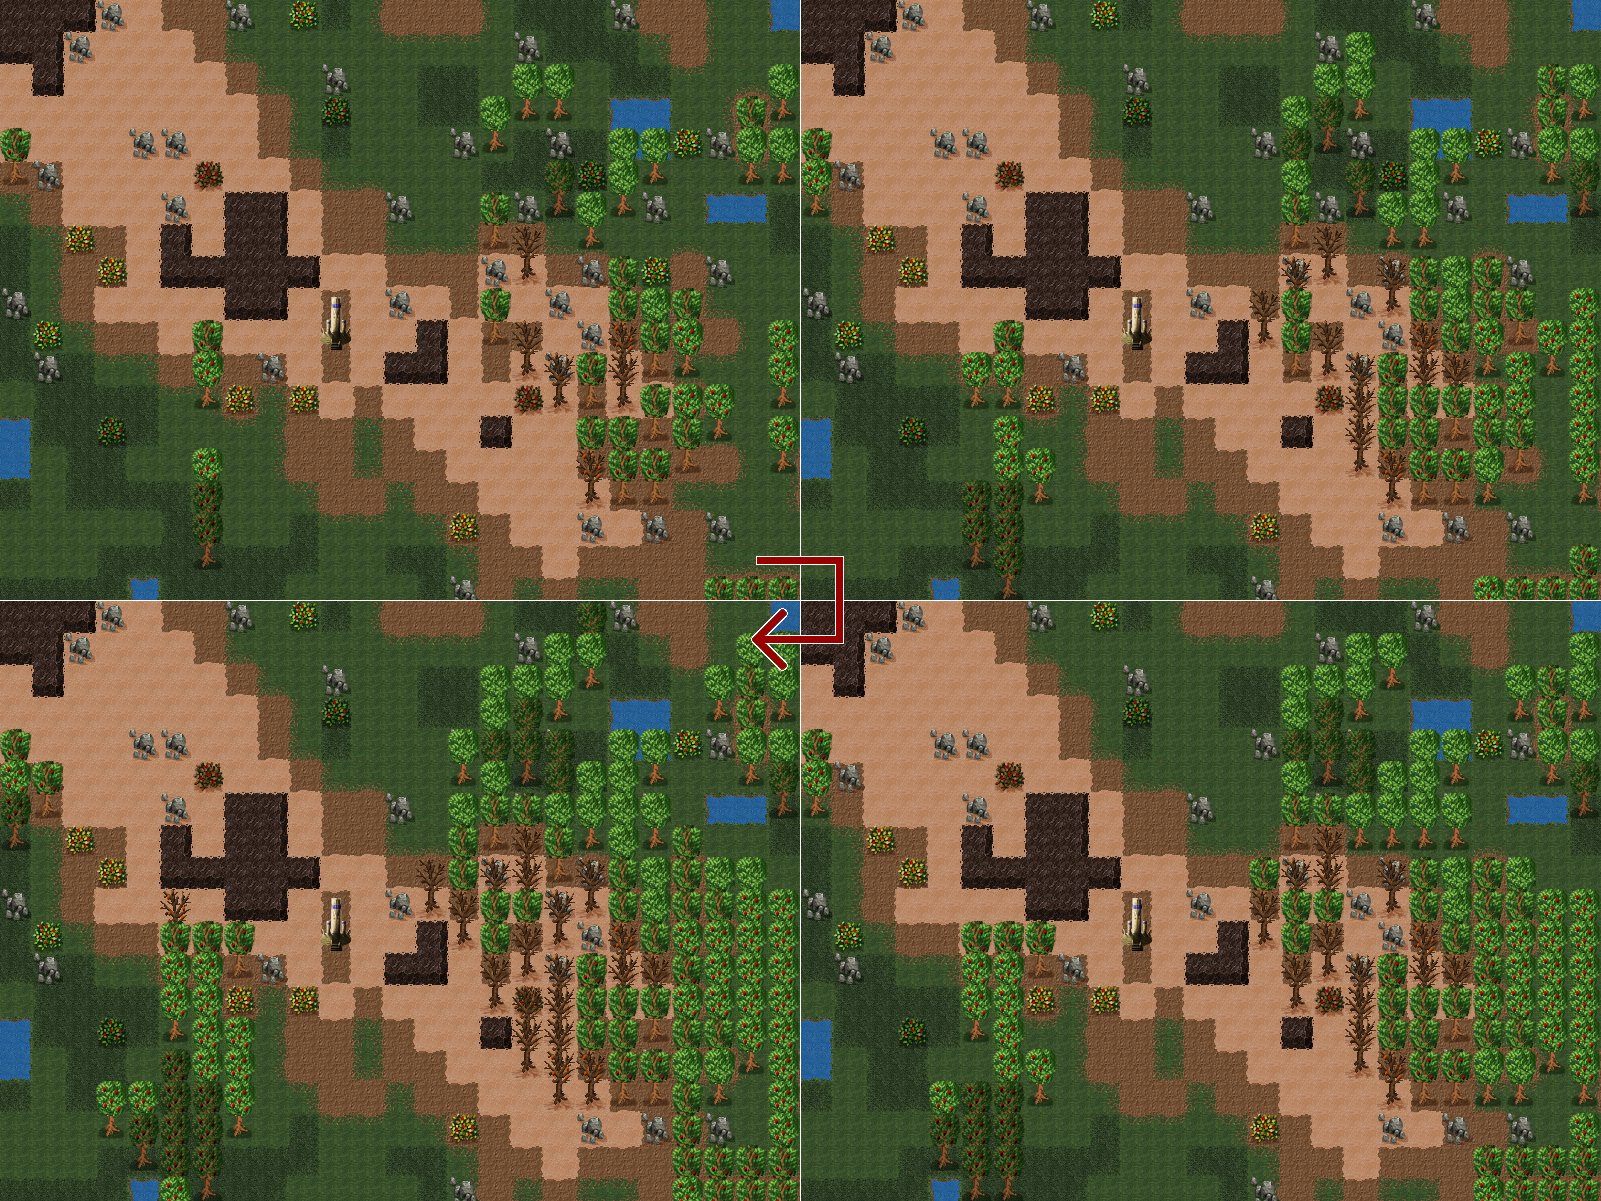
\includegraphics[scale=0.45]{img/DilateForest.png}
        \end{center}
        \caption{Dilatation des forêts}
      \end{figure}
      \begin{figure}
        \begin{center}
          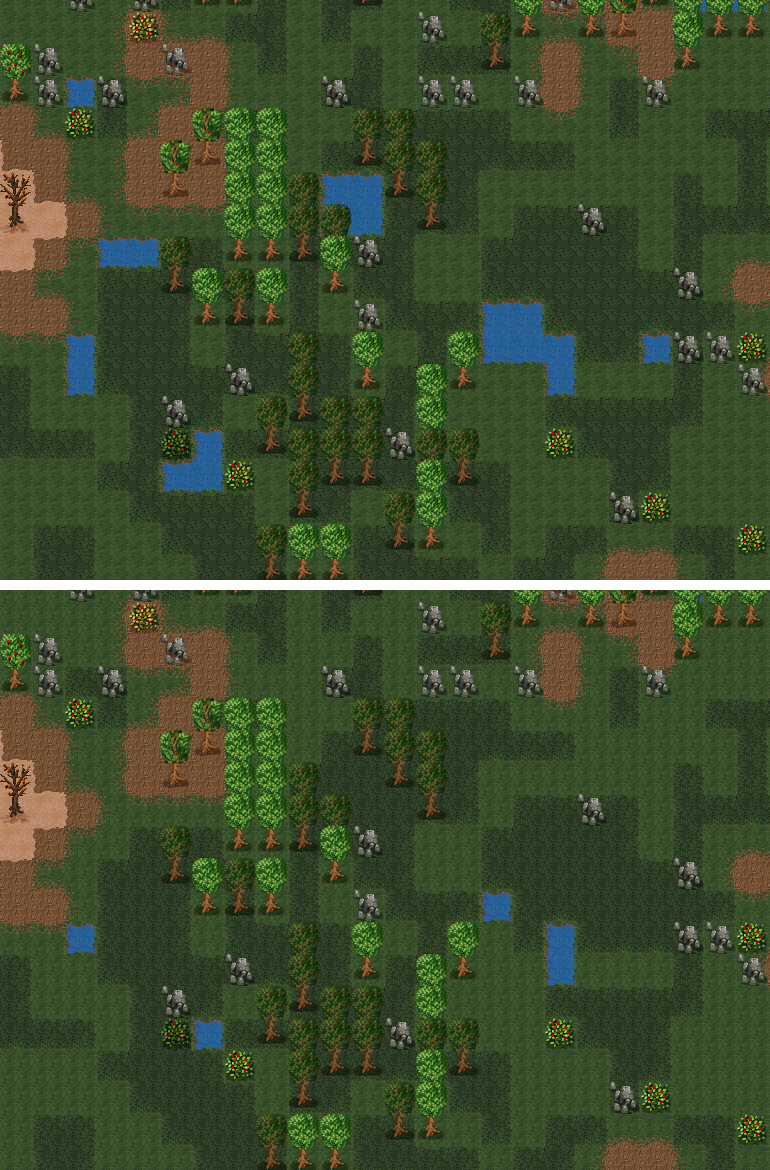
\includegraphics[scale=0.45]{img/ErodeFluid.png}
        \end{center}
        \caption{Erosion des étendues de fluides}
      \end{figure}
      \begin{figure}
        \begin{center}
          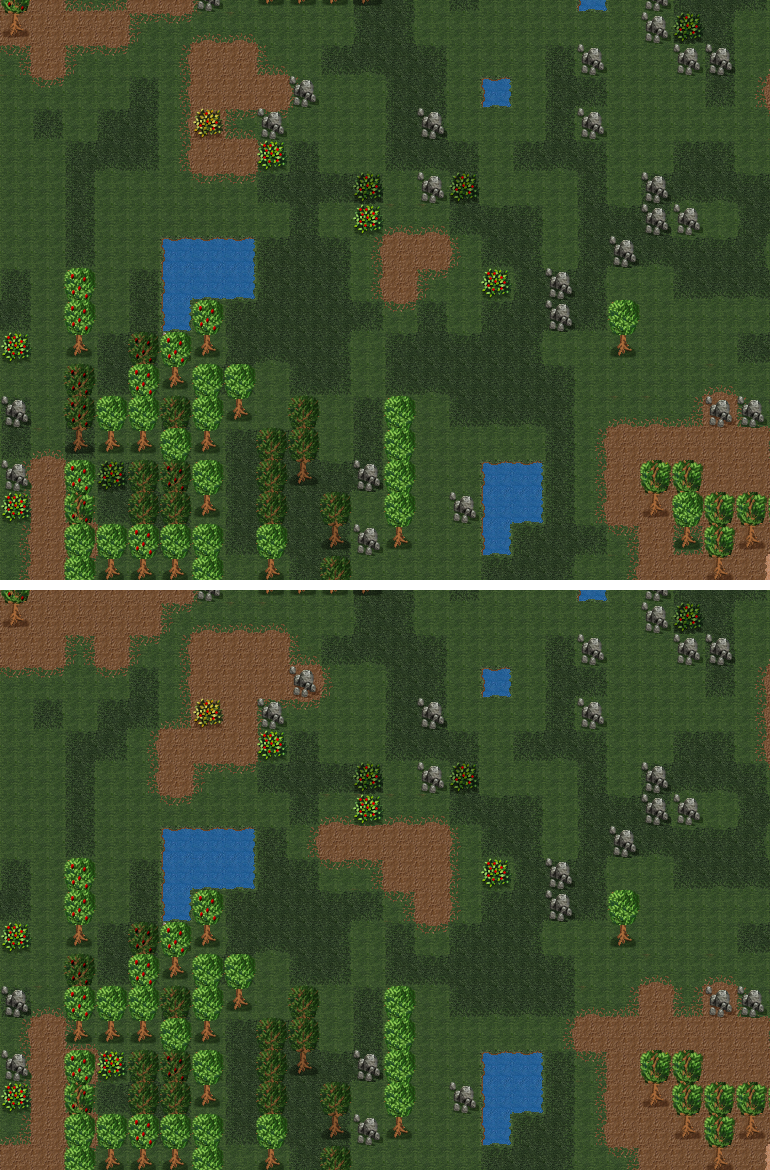
\includegraphics[scale=0.45]{img/ErodeNearFluid.png}
        \end{center}
        \caption{Erosion des zones humides}
      \end{figure}
      \begin{figure}
        \begin{center}
          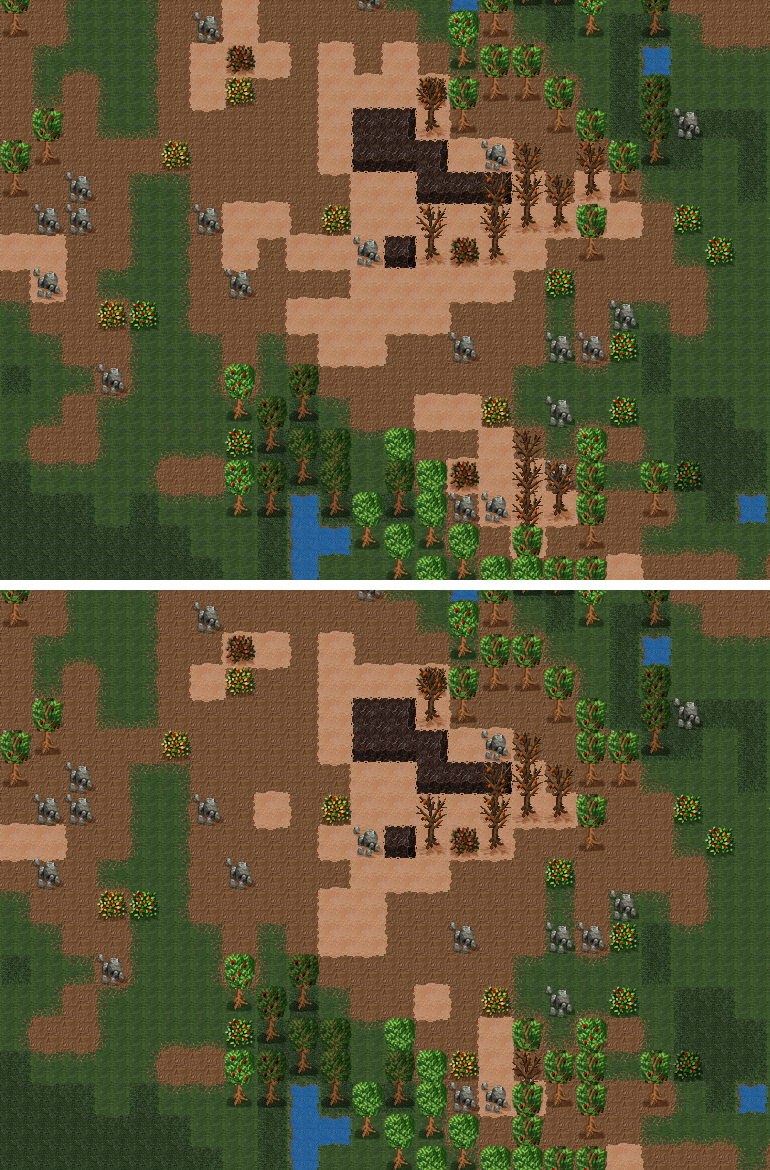
\includegraphics[scale=0.45]{img/ErodeNearCliff.png}
         \end{center}
        \caption{Erosion des zones sèches}
      \end{figure}
      \begin{figure}
        \begin{center}
          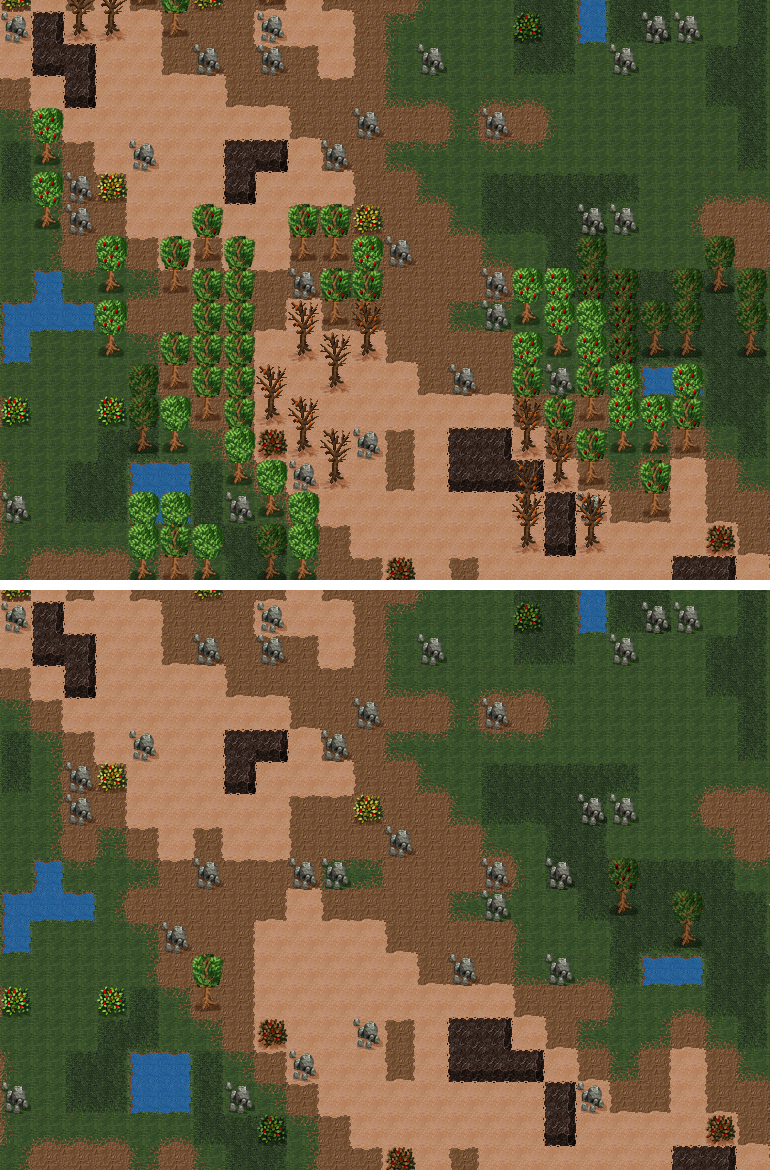
\includegraphics[scale=0.45]{img/ErodeForest.png}
        \end{center}
        \caption{Erosion des forêts}
      \end{figure}
      \begin{figure}
        \begin{center}
          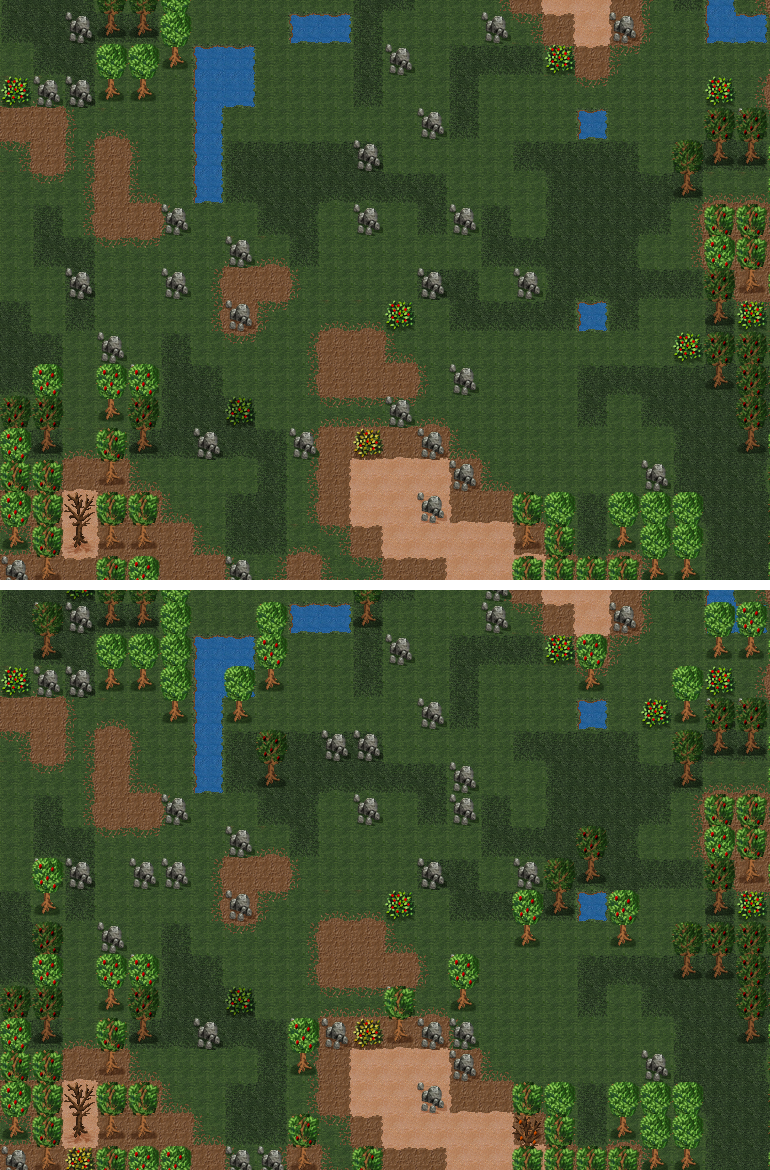
\includegraphics[scale=0.45]{img/SpawnRessource.png}
        \end{center}
        \caption{Apparition de tout type de ressource}
      \end{figure}
      \begin{figure}
        \begin{center}
          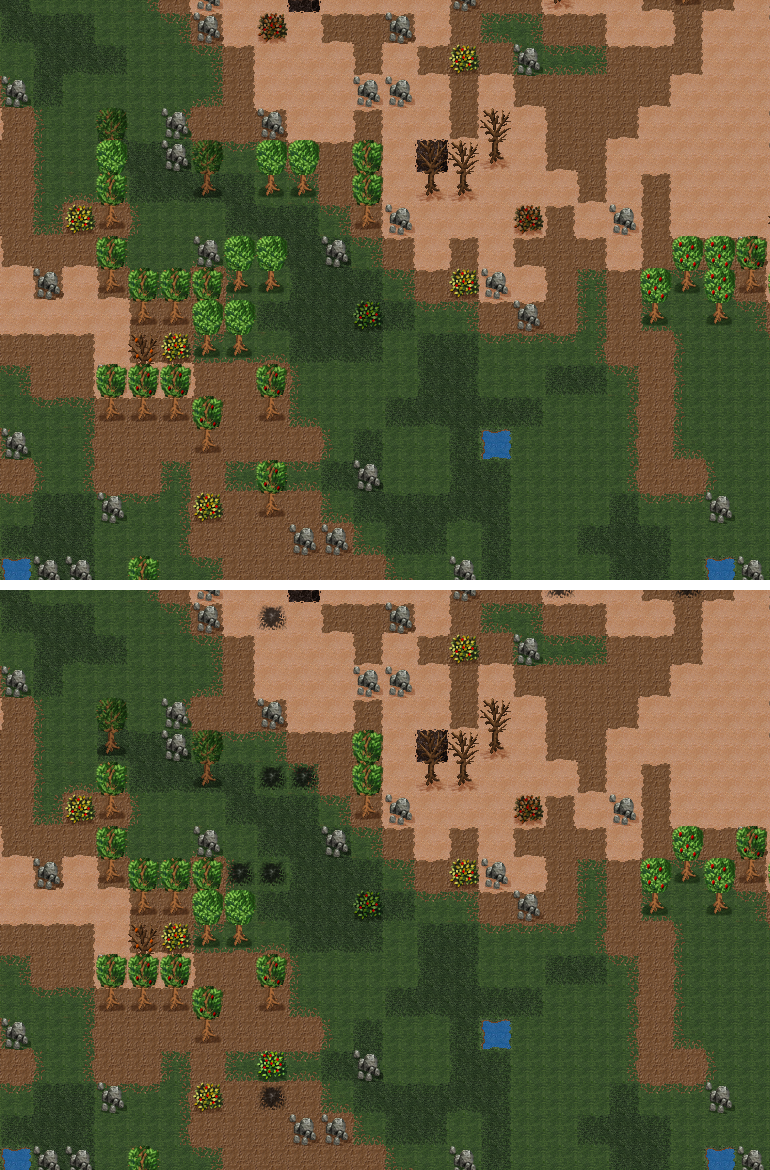
\includegraphics[scale=0.45]{img/BurnRessource.png}
        \end{center}
        \caption{Disparition par le feu des ressources contenant du bois}
      \end{figure}
      \begin{figure}
        \begin{center}
          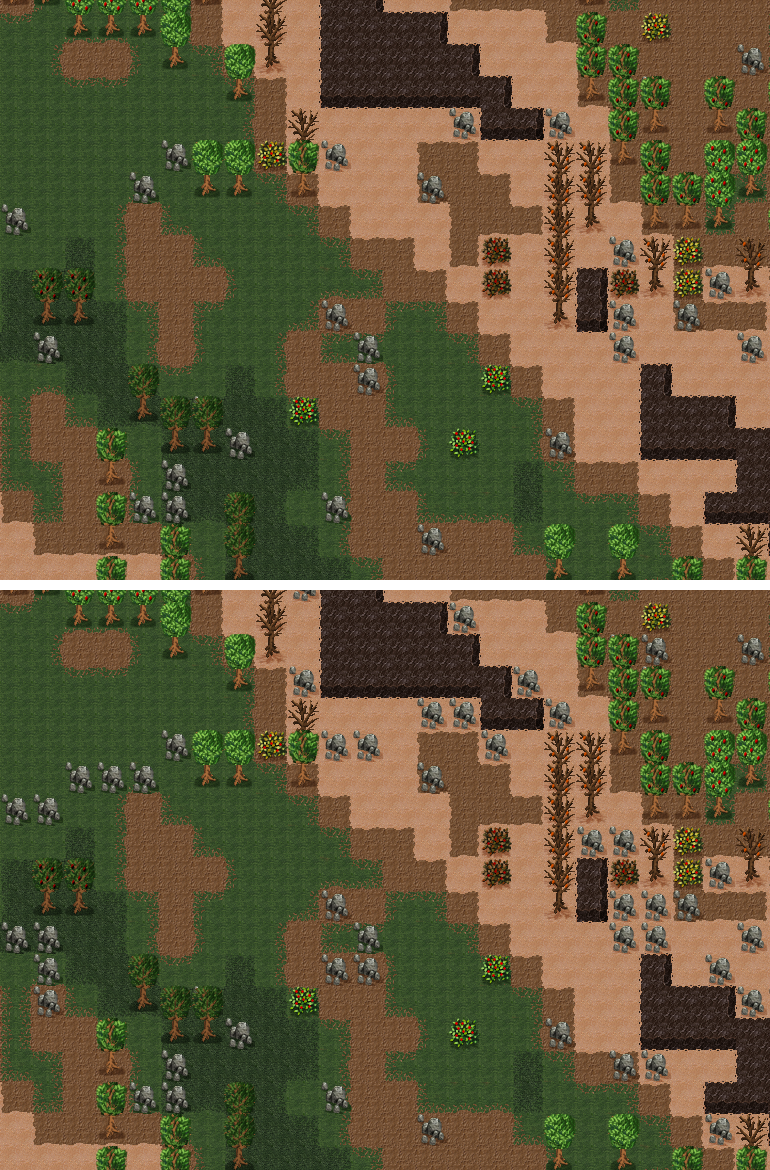
\includegraphics[scale=0.45]{img/SpawnOnlyStone.png}
        \end{center}
        \label{IncidenceFin}
        \caption{Apparition de rochers uniquement}
      \end{figure}

\end{document}
